\documentclass{beamer}

% % % % % % % % % % % % % % % % % % % % 
% Preblem
%
\usetheme{metropolis}
\usepackage[backend=bibtex,style=authoryear]{biblatex}
\usepackage{listings}
\addbibresource{references.bib}

% add commar between name and year \ Default (Name Year), Renew (Name, Year)
\renewcommand*{\nameyeardelim}{\addcomma\addspace}

% - - - - - - - - - - - - - - - - - - - -
% NEED BY \makethesiscover
% - - - - - - - - - - - - - - - - - - - -
% Common
\newcommand{\studentEmailaddress}{sitdhibong.l@student.chula.ac.th}
% English letters
\newcommand{\ThesisNameEN}{Test Case Generation from a Java Static Call Graph}
\newcommand{\authorNameEN}{Sitdhibong Laokok}
\newcommand{\prefixEN}{Mr.}
\newcommand{\studentnameEn}{{\prefixEN}~{\authorNameEN}}
\newcommand{\curriculumnEn}{Master of Science}
\newcommand{\majorEn}{Software Engineering}
\newcommand{\departmentEn}{Computer Engineering}
\newcommand{\facultyEn}{Faculty of Engineering}
\newcommand{\universityEn}{Chulalongkorn University}
\newcommand{\disclaiminationEn}{Copyright Year 2016}
\newcommand{\advisorEn}{Taratip Suwannasart}
\newcommand{\engkeywords}{Test case generation, Java language, Static call graph}
\newcommand{\academicYearEn}{2016}


\usepackage[font=scriptsize]{caption}
\usepackage{mwe}

\definecolor{brewcolorRed}{RGB}{150,4,12}

\setbeamercolor{frametitle}{fg=white,bg=brewcolorRed}

\metroset{%
    progressbar=head
}

\defbeamertemplate*{footline}{}%
{
    \leavevmode%
    \hbox{%
        \begin{beamercolorbox}[wd=.3\paperwidth,ht=2ex,dp=2ex,center]{section in footer}%
            
\includegraphics[width=0.25\paperwidth]{figure/chula-engineering}
        \end{beamercolorbox}

        \begin{beamercolorbox}[wd=.5\paperwidth,ht=2ex,dp=2ex,center]{subsection in footer}%
            \insertsubsection
            \vspace{0.2cm}
        \end{beamercolorbox}

        \begin{beamercolorbox}[wd=.2\paperwidth,ht=6ex,dp=2ex,right]{pagenumber in footer}%
            \vfill
            \insertframenumber{}\hspace{1cm}
            \vspace{0.2cm}
        \end{beamercolorbox}
    }
}

% % % % % % % % % % % % % % % % % % % % 

% % % % % % % % % % % % % % % % % % % % 
% Title config
%
\title{\ThesisNameEN}
\subtitle{IMECS2017}
\date[2017.03.14]{\today}
\author{\authorNameEN~\small{and~\advisorEn}}
\institute{{\facultyEn}, {\universityEn}}
% % % % % % % % % % % % % % % % % % % % 

\begin{document}

\maketitle

\begin{frame}[t]{Outline}
    \tableofcontents[hideallsubsections]
\end{frame}

\newcommand{\displayframe}{%
    \begin{frame}{Outline}
    \tableofcontents[%
        currentsection,
        subsectionstyle=hide
        ]
    \end{frame}
}
% % % % % % % % % % % % % % % % % % % % 
% Introduction
%
\section{Introduction}
\begin{frame}{Software Testing's benefits}
  \begin{itemize}
     \item Indicating the confidencial level of Software Under Test
     \item Verifying conformance to Software Requirements Specification
     \item Discovering errors in source code
  \end{itemize}
\end{frame}

\begin{frame}{Various Platforms}
    \begin{figure}
        \includegraphics[width=.8\paperwidth]{figure/mobile_bugs}
        \caption{Various platforms for software}
        \label{fig:variousplatform}
    \end{figure}
\end{frame}

\begin{frame}{Various of Languages}
    \begin{figure}
        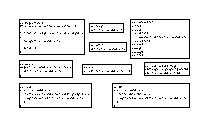
\includegraphics[width=.9\paperwidth]{figure/hello-world-lang}
        \caption{$Hello~World!$ in difference languages}
        \label{fig:helloworld}
    \end{figure}
    \note{Hello world}
\end{frame}

\begin{frame}{Software contains modules}
    \begin{figure}
        
\includegraphics[width=.7\paperwidth]{figure/software-modules}
        \caption{Software modules}
        \label{fig:softwareModules}
    \end{figure}
\end{frame}

\begin{frame}{Software works together}
    \begin{figure}
        \includegraphics[height=.7\paperheight]{figure/graph.png}
        \caption{Connections between Classes}
        \label{fig:classConnection}
        % http://nion.modprobe.de/blog/archives/556-creating-dynamic-function-call-graphs.html
    \end{figure}
\end{frame}

% \begin{frame}{Faults Detection Metric}
%     \begin{figure}
%         \begin{equation}
%             APFD~=~1-~\frac{\sum^{num_f}_{i=1}{TF_i}}{{num}_t \cdot {num}_f} %
%                     +~\frac{1}{2 \cdot {num}_t}
%             \label{eq:apfd}
%         \end{equation}
%         \caption{Average Percentage Faults Detected metric \parencite{792604}}
%         \label{fig:apfd}
%     \end{figure}
% \end{frame}

% % % % % % % % % % % % % % % % % % % % 

% % % % % % % % % % % % % % % % % % % % 
% Related works
%
% \section{Related works}
% \begin{frame}{Automatic Test Case Generation Using Sequence Diagram}
% \end{frame}
% 
% \begin{frame}{Data flow based Test Case Generation Algorithm for Object Oriented Integration Testing}
% \end{frame}
% % % % % % % % % % % % % % % % % % % % 

% % % % % % % % % % % % % % % % % % % % 
% Background
%
\section{Background}
\subsection{Program graph}
\begin{frame}{Program graph}
    \begin{enumerate}
        \item Control Flow Graph
        \item Static Call Graph
    \end{enumerate}
\end{frame}


\begin{frame}{Control Flow Graph}
    \begin{figure}
        
\includegraphics[width=.8\paperwidth]{figure/Primitive-Operation-Structure}
        \caption{Primitive operation structure \parencite{McCabe1976}}
        \label{fig:primitivestructure}
    \end{figure}
\end{frame}

\begin{frame}{Source Code Structure}
    % \textbf{Control flow graph definition}
    % \parencite{Allen:1970:CFA:390013.808479}
    \begin{figure}
        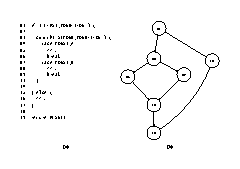
\includegraphics[height=.7\paperheight]{figure/cfg-transform}
        \caption{Source code transformation: (a) Source code (b) Control Flow Graph}
        \label{fig:sourceCodeTransf}
        % http://nion.modprobe.de/blog/archives/556-creating-dynamic-function-call-graphs.html
    \end{figure}
\end{frame}

\begin{frame}{Program Graph}
    \begin{enumerate}
        \item<1-> Control Flow Graph
        \item<2-> Static Call Graph
    \end{enumerate}
\end{frame}

\begin{frame}{Software are composed by classes}
    \begin{figure}
        
\includegraphics[width=0.6\paperwidth]{figure/class-connected}
        \caption{Class connection}
        \label{fig:classConnect}
    \end{figure}
\end{frame}

\begin{frame}{Class interfaces}
    \begin{figure}
        
\includegraphics[height=0.6\paperheight]{figure/class-interfaces}
        \caption{Class Interfaces between Class A and B}
        \label{fig:classInterfaces}
    \end{figure}
\end{frame}

\begin{frame}{Static Call Graph}
    \begin{figure}
        
\includegraphics[width=0.8\paperwidth]{figure/SCG-A-and-B}
        \caption{Static Call Graph of Class A and B}
        \label{fig:staticCallGraphAandB}
    \end{figure}
\end{frame}

% % % % % % % % % % % % % % % % % % % % 

% % % % % % % % % % % % % % % % % % % % 
% Proposed approach
%
% \section{Related works}
% \begin{frame}{First}
%     she \parencite{Panthi2012}
% \end{frame}
% 
% \begin{frame}{Second}
%     he \parencite{7339088}
% \end{frame}

% % % % % % % % % % % % % % % % % % % % 

% % % % % % % % % % % % % % % % % % % % 
% Proposed approach
%
\section{Proposed Approach}
\subsection{Methodology}
% \begin{frame}{Methodology overview}
\begin{frame}
    \begin{figure}
        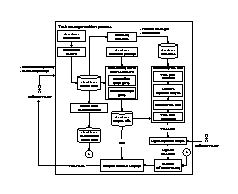
\includegraphics[height=0.8\paperheight]{figure/Methodology}
        \caption{Methodology of Test Case Generation based on Static Data}
        \label{fig:methodologyOverview}
    \end{figure}
\end{frame}

\subsection{Constant collection}
\begin{frame}{Constant collection}
    \begin{figure}
        \includegraphics[width=0.8\paperwidth]{figure/constants-collection.pdf}
        \caption{Constants Collection in the Class}
        \label{fig:constantsCollection}
    \end{figure}
\end{frame}

\subsection{Constructing source code's structure}
\begin{frame}{Constructing source code's structure}
    \begin{figure}
        \includegraphics[width=0.9\paperwidth]{figure/cfg-construction.pdf}
        \caption{Control Flow Graph Construction from Source Code}
        \label{fig:cfgConstruct}
    \end{figure}
\end{frame}

\begin{frame}{Constructing source code's structure}
    \begin{figure}
        \includegraphics[width=0.7\paperwidth]{figure/scg-construction.pdf}
        \caption{Static Call Graph Construction from Classes}
        \label{fig:scgConstruct}
    \end{figure}
\end{frame}

\begin{frame}{Static Call Graph form}
    \begin{figure}
        \includegraphics[width=0.7\paperwidth]{figure/scg-form.pdf}
        \caption{Static Call Graph Form between the Interfaces of Classes}
        \label{fig:scgForm}
    \end{figure}
\end{frame}

\subsection{Source code instrumentation}
\begin{frame}{Source code instrumentation}
    \begin{itemize}
        \item<1-> Code Coverage Indentification
        \item<2-> Run-time Tracking
    \end{itemize}
\end{frame}

\subsection{Summarization}
\begin{frame}{Summarization}
    \begin{itemize}
        \item Understand source code structure
        \item Collection of constant in source code
        \item Instrumented code for execute generated test cases
    \end{itemize}
\end{frame}

\subsection{Generating Test case}
\begin{frame}
    \begin{figure}
        \includegraphics<1>[height=0.8\paperheight]{figure/Methodology}
        \includegraphics<2>[height=0.8\paperheight]{figure/Methodology-Highlight-1}
    \end{figure}
\end{frame}

\begin{frame}
    \begin{figure}
        \includegraphics[height=.8\paperheight]{figure/Activities}
        \caption{Test case generation}
        \label{fig:testcasegenearation}
    \end{figure}
\end{frame}

\begin{frame}{Selecting test path}
    \begin{figure}
        \includegraphics<1>[width=.8\paperwidth]{figure/psuedo-classes-connection}
        \caption{Class's structure}
        \label{fig:classStructure}
    \end{figure}
\end{frame}

\begin{frame}{Selecting test path}
    \begin{figure}
        \includegraphics<1>[width=.8\paperwidth]{figure/Relationship-between-Classes}
        \includegraphics<2>[width=.8\paperwidth]{figure/3rd-test-path}
        \includegraphics<3>[width=.8\paperwidth]{figure/2nd-test-path}
        \includegraphics<4>[width=.8\paperwidth]{figure/1st-test-path}
        \caption{Relation of Classes}
        \label{fig:relationOfClassInSCGForm}
    \end{figure}
\end{frame}

\begin{frame}{Selecting test paths}
    \begin{figure}
        \includegraphics<1>[height=.6\paperheight]{figure/Calling-statements-of-Classes}
        \includegraphics<2>[height=.6\paperheight]{figure/Calling-statements-of-Classes-1}
        \includegraphics<3>[height=.6\paperheight]{figure/Calling-statements-of-Classes-2}
        \includegraphics<4>[height=.6\paperheight]{figure/Calling-statements-of-Classes-3}
        \includegraphics<5>[height=.6\paperheight]{figure/Calling-statements-of-Classes-4}
        \includegraphics<6>[height=.6\paperheight]{figure/Calling-statements-of-Classes-5}
        \includegraphics<7>[height=.6\paperheight]{figure/Calling-statements-of-Classes-6}
        \caption{Calling Statement between Method $m_{11}$, $m_{21}$ and $m_{31}$ of Class $C_1$, $C_2$ and $C_3$ respectively }
        \label{fig:testcasegenearation}
    \end{figure}
\end{frame}

\begin{frame}{Analizing method signature}
    \centering
    \makebox[0.7\paperwidth][l]{$m_{11}~:~12~~studentScore~>80$}
    \makebox[0.7\paperwidth][l]{$m_{11}~:~14~~studentScore~>50$}
    \makebox[0.7\paperwidth][l]{$m_{21}~:~11~~true~>~hasQuizScore$}
\end{frame}

\begin{frame}{Analizing method signature}
    \centering
    \makebox[0.7\paperwidth][l]{$m_{11}(String~studntID,~float~studentScore)~:~String$}
    \makebox[0.7\paperwidth][l]{$m_{11}(String~studentID)~:~float$}
    \makebox[0.7\paperwidth][l]{$m_{21}(String~studentID)~:~float$}
\end{frame}

\begin{frame}
    \begin{figure}
        \includegraphics[width=0.8\paperwidth]{figure/constants-collection.pdf}
    \end{figure}
\end{frame}

\begin{frame}{Generating test case}
    \begin{figure}
        \includegraphics<1>[height=0.8\paperheight]{figure/Methodology}
        \includegraphics<2>[height=0.8\paperheight]{figure/Methodology-Highlight-1}
    \end{figure}
\end{frame}

\subsection{Adjust expected output}
\begin{frame}{Adjust expected output}
    \begin{figure}
        \includegraphics<1>[width=.8\paperwidth]{figure/example-of-generated-test-case.pdf}
        \includegraphics<2>[width=.8\paperwidth]{figure/adjusted-example-of-generated-test-case.pdf}
        \caption{Gnerated test case}
        \label{fig:classStructure}
    \end{figure}
\end{frame}

\subsection{Final phase}
\begin{frame}
    \begin{figure}
        \includegraphics[height=0.8\paperheight]{figure/Methodology-Highlight-2}
    \end{figure}
\end{frame}
% % % % % % % % % % % % % % % % % % % % 

% % % % % % % % % % % % % % % % % % % % 
% Conclusion
%
\section{Conclusion}
\begin{frame}{Conclusion}
    \begin{itemize}
        \item<1->Introduce an approach for test case generation based on integration testing by considering the static call graph.
        \item<2->Generated test cases exercise all branches in the graph, branch coverage.
        \item<3->Test data also prepaire to make the test case exercise throught the selected test paths.
    \end{itemize}
\end{frame}
% % % % % % % % % % % % % % % % % % % % 

% % % % % % % % % % % % % % % % % % % % 
% Conclusion
%
\begin{frame}
    \Large{Question \& Answer}
\end{frame}
% % % % % % % % % % % % % % % % % % % % 
\end{document}
